\section{Additional Configuration}
\label{sec:Additional_Configuration}


\subsection{Configure SSH passwordless}
By default, COMPSs uses SSH libraries for communication between nodes. Consequently, after COMPSs is installed on a set of machines,
the SSH keys must be configured on those machines so that COMPSs can establish passwordless connections between them. This requires
to install the OpenSSH package (if not present already) and follow these steps \textbf{in each machine}:
\begin{enumerate}
 \item Generate an SSH key pair
       \begin{lstlisting}[language=bash]
	  $ ssh-keygen -t dsa
       \end{lstlisting}
 \item Distribute the public key to all the other machines and configure it as authorized
       \begin{lstlisting}[language=bash]
          For every other available machine (MACHINE):
	  $ scp ~/.ssh/id_dsa.pub MACHINE:./myDSA.pub
	  $ ssh MACHINE "cat ./myDSA.pub >> ~/.ssh/authorized_keys; rm ./myDSA.pub"
       \end{lstlisting}
 \item Check that passwordless SSH connections are working fine
       \begin{lstlisting}[language=bash]
          For every other available machine (MACHINE):
	  $ ssh MACHINE
       \end{lstlisting}
\end{enumerate}

For example, considering the cluster shown in Figure \ref{fig:cluster}, users will have to execute the following commands
to grant free ssh access between any pair of machines:
\begin{lstlisting}[language=bash]
 me@localhost:~$ ssh-keygen -t id_dsa
 # Granting access localhost -> m1.bsc.es
 me@localhost:~$ scp ~/.ssh/id_dsa.pub user_m1@m1.bsc.es:./me_localhost.pub
 me@localhost:~$ ssh user_m1@m1.bsc.es "cat ./me_localhost.pub >> ~/.ssh/authorized_keys; rm ./me_localhost.pub"
 # Granting access localhost -> m2.bsc.es
 me@localhost:~$ scp ~/.ssh/id_dsa.pub user_m2@m2.bsc.es:./me_localhost.pub
 me@localhost:~$ ssh user_m2@m2.bsc.es "cat ./me_localhost.pub >> ~/.ssh/authorized_keys; rm ./me_localhost.pub"
 
 me@localhost:~$ ssh user_m1@m1.bsc.es
 user_m1@m1.bsc.es:~> ssh-keygen -t id_dsa
 user_m1@m1.bsc.es:~> exit
 # Granting access m1.bsc.es -> localhost
 me@localhost:~$ scp user_m1@m1.bsc.es:~/.ssh/id_dsa.pub ~/userm1_m1.pub
 me@localhost:~$ cat ~/userm1_m1.pub >> ~/.ssh/authorized_keys
 # Granting access m1.bsc.es -> m2.bsc.es
 me@localhost:~$ scp ~/userm1_m1.pub user_m2@m2.bsc.es:~/userm1_m1.pub 
 me@localhost:~$ ssh user_m2@m2.bsc.es "cat ./userm1_m1.pub >> ~/.ssh/authorized_keys; rm ./userm1_m1.pub"
 me@localhost:~$ rm ~/userm1_m1.pub
 
 me@localhost:~$ ssh user_m2@m2.bsc.es
 user_m2@m2.bsc.es:~> ssh-keygen -t id_dsa
 user_m2@m2.bsc.es:~> exit
 # Granting access m2.bsc.es -> localhost
 me@localhost:~$ scp user_m2@m1.bsc.es:~/.ssh/id_dsa.pub ~/userm2_m2.pub
 me@localhost:~$ cat ~/userm2_m2.pub >> ~/.ssh/authorized_keys
 # Granting access m2.bsc.es -> m1.bsc.es
 me@localhost:~$ scp ~/userm2_m2.pub user_m1@m1.bsc.es:~/userm2_m2.pub 
 me@localhost:~$ ssh user_m1@m1.bsc.es "cat ./userm2_m2.pub >> ~/.ssh/authorized_keys; rm ./userm2_m2.pub"
 me@localhost:~$ rm ~/userm2_m2.pub
\end{lstlisting}

\begin{figure}[h!]
  \centering
    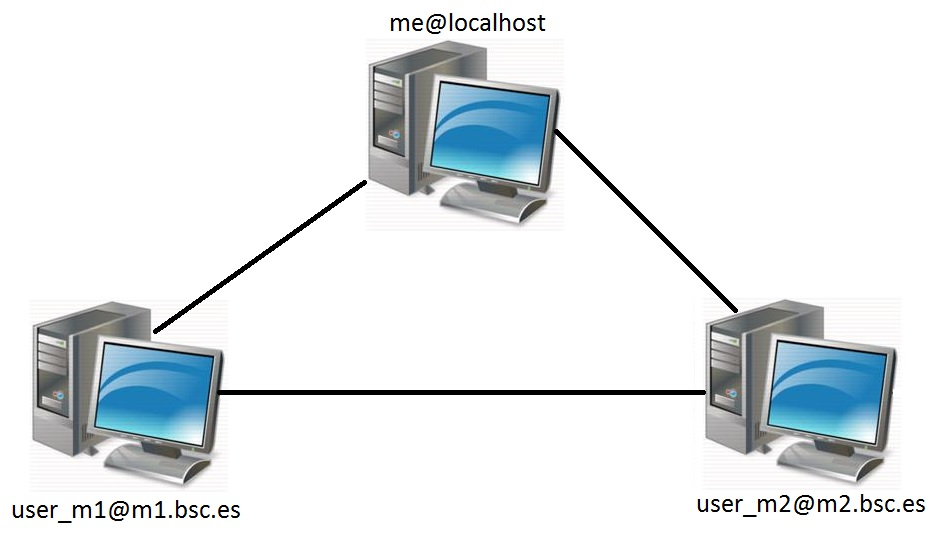
\includegraphics[width=0.95\textwidth]{./Sections/7_Additional_Configuration/Figures/cluster.jpeg}
    \caption{Cluster example}
    \label{fig:cluster}
\end{figure}

\subsection{Configure the COMPSs Cloud Connectors}
This section provides information about the additional configuration needed for some Cloud Connectors.

\subsubsection{OCCI (Open Cloud Computing Interface) connector}
In order to execute a COMPSs application using cloud resources, the rOCCI (Ruby OCCI) connector has to be configured properly.
The connector uses the rOCCI CLI client (upper versions from 4.2.5) which has to be installed in the node where the COMPSs main
application runs. The client can be installed following the instructions detailed at 
\url{http://appdb.egi.eu/store/software/rocci.cli}